\chapter{欧拉图}
\begin{Def}
包含图的所有顶点和所有边的闭迹称为{\bfseries 欧拉闭迹}。存在一条欧拉闭迹的图称为
{\bfseries 欧拉图}。
\end{Def}

\begin{Def}
  包含图的所有顶点和边的迹称为{\bfseries 欧拉迹}。
\end{Def}



\begin{Ex}
图G是欧拉图当且仅当$G$是连通的且每个顶点的度是偶数。
\end{Ex}
\begin{Ex}
图G有一条欧拉开迹当且仅当$G$是连通的且恰有两个奇度顶点。  
\end{Ex}
\begin{Ex}
      设$G$是连通图,$G$恰有$2n$个奇度顶点,$n \geq 1$,证明$G$的全部边可以排成$n$
      条开迹,且不能排成少于$n$条开迹。
\end{Ex}


\begin{Ex}
  以下4个图中,存在欧拉闭迹的是$\underline{\quad\quad}$。
  \vspace{0.5cm}

  A.
    \begin{minipage}{0.18\linewidth}
    \centering
    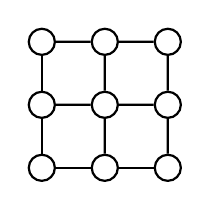
\begin{tikzpicture}[auto,
    specification/.style ={circle, draw, thick}, scale = 0.8]
   \node[specification] (A)  at (0,0)  {};
   \node[specification] (B)  at (1,0)  {};
   \node[specification] (C)  at (2,0)  {};
   \node[specification] (D)  at (0,1)  {};
   \node[specification] (E)  at (1,1)  {};
   \node[specification] (F)  at (2,1)  {};
   \node[specification] (G)  at (0,2)  {};
   \node[specification] (H)  at (1,2)  {};
   \node[specification] (I)  at (2,2)  {};

   \draw[thick] (A) to  (B);
   \draw[thick] (B) to  (C);
   \draw[thick] (D) to  (E);
   \draw[thick] (E) to  (F);
   \draw[thick] (G) to (H);
   \draw[thick] (H) to (I);
   \draw[thick] (A) to (D);
   \draw[thick] (B) to (E);
   \draw[thick] (C) to (F);
   \draw[thick] (D) to (G);
   \draw[thick] (E) to (H);
   \draw[thick] (F) to (I);
 \end{tikzpicture}
\end{minipage}\hfill
  B.
    \begin{minipage}{0.18\linewidth}
    \centering
    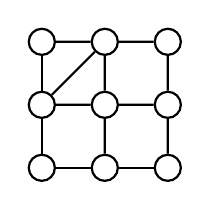
\begin{tikzpicture}[auto,
    specification/.style ={circle, draw, thick}, scale = 0.8]
   \node[specification] (A)  at (0,0)  {};
   \node[specification] (B)  at (1,0)  {};
   \node[specification] (C)  at (2,0)  {};
   \node[specification] (D)  at (0,1)  {};
   \node[specification] (E)  at (1,1)  {};
   \node[specification] (F)  at (2,1)  {};
   \node[specification] (G)  at (0,2)  {};
   \node[specification] (H)  at (1,2)  {};
   \node[specification] (I)  at (2,2)  {};

   \draw[thick] (A) to  (B);
   \draw[thick] (B) to  (C);
   \draw[thick] (D) to  (E);
   \draw[thick] (E) to  (F);
   \draw[thick] (G) to (H);
   \draw[thick] (H) to (I);
   \draw[thick] (A) to (D);
   \draw[thick] (B) to (E);
   \draw[thick] (C) to (F);
   \draw[thick] (D) to (G);
   \draw[thick] (E) to (H);
   \draw[thick] (F) to (I);
   \draw[thick] (D) to (H);

 \end{tikzpicture}
\end{minipage}\hfill
      C.
    \begin{minipage}{0.18\linewidth}
    \centering
    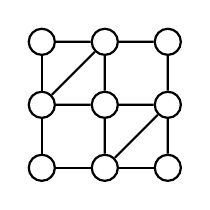
\begin{tikzpicture}[auto,
    specification/.style ={circle, draw, thick}, scale=0.8]
   \node[specification] (A)  at (0,0)  {};
   \node[specification] (B)  at (1,0)  {};
   \node[specification] (C)  at (2,0)  {};
   \node[specification] (D)  at (0,1)  {};
   \node[specification] (E)  at (1,1)  {};
   \node[specification] (F)  at (2,1)  {};
   \node[specification] (G)  at (0,2)  {};
   \node[specification] (H)  at (1,2)  {};
   \node[specification] (I)  at (2,2)  {};

   \draw[thick] (A) to  (B);
   \draw[thick] (B) to  (C);
   \draw[thick] (D) to  (E);
   \draw[thick] (E) to  (F);
   \draw[thick] (G) to (H);
   \draw[thick] (H) to (I);
   \draw[thick] (A) to (D);
   \draw[thick] (B) to (E);
   \draw[thick] (C) to (F);
   \draw[thick] (D) to (G);
   \draw[thick] (E) to (H);
   \draw[thick] (F) to (I);
   \draw[thick] (D) to (H);
   \draw[thick] (B) to (F);
 \end{tikzpicture}
\end{minipage}\hfill
      D.
    \begin{minipage}{0.18\linewidth}
    \centering
    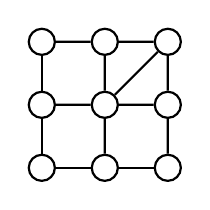
\begin{tikzpicture}[auto,
    specification/.style ={circle, draw, thick}, scale=0.8]
   \node[specification] (A)  at (0,0)  {};
   \node[specification] (B)  at (1,0)  {};
   \node[specification] (C)  at (2,0)  {};
   \node[specification] (D)  at (0,1)  {};
   \node[specification] (E)  at (1,1)  {};
   \node[specification] (F)  at (2,1)  {};
   \node[specification] (G)  at (0,2)  {};
   \node[specification] (H)  at (1,2)  {};
   \node[specification] (I)  at (2,2)  {};

   \draw[thick] (A) to  (B);
   \draw[thick] (B) to  (C);
   \draw[thick] (D) to  (E);
   \draw[thick] (E) to  (F);
   \draw[thick] (G) to (H);
   \draw[thick] (H) to (I);
   \draw[thick] (A) to (D);
   \draw[thick] (B) to (E);
   \draw[thick] (C) to (F);
   \draw[thick] (D) to (G);
   \draw[thick] (E) to (H);
   \draw[thick] (F) to (I);
   \draw[thick] (E) to (I);

 \end{tikzpicture}
\end{minipage}\hfill

\end{Ex}

\begin{Ex}
  以下4个图中,存在一条欧拉开迹的是$\underline{\quad\quad}$。
  \vspace{0.5cm}

  A.
    \begin{minipage}{0.18\linewidth}
    \centering
    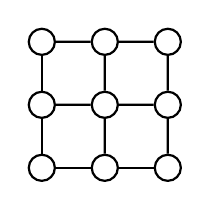
\begin{tikzpicture}[auto,
    specification/.style ={circle, draw, thick}, scale = 0.8]
   \node[specification] (A)  at (0,0)  {};
   \node[specification] (B)  at (1,0)  {};
   \node[specification] (C)  at (2,0)  {};
   \node[specification] (D)  at (0,1)  {};
   \node[specification] (E)  at (1,1)  {};
   \node[specification] (F)  at (2,1)  {};
   \node[specification] (G)  at (0,2)  {};
   \node[specification] (H)  at (1,2)  {};
   \node[specification] (I)  at (2,2)  {};

   \draw[thick] (A) to  (B);
   \draw[thick] (B) to  (C);
   \draw[thick] (D) to  (E);
   \draw[thick] (E) to  (F);
   \draw[thick] (G) to (H);
   \draw[thick] (H) to (I);
   \draw[thick] (A) to (D);
   \draw[thick] (B) to (E);
   \draw[thick] (C) to (F);
   \draw[thick] (D) to (G);
   \draw[thick] (E) to (H);
   \draw[thick] (F) to (I);
 \end{tikzpicture}
\end{minipage}\hfill
  B.
    \begin{minipage}{0.18\linewidth}
    \centering
    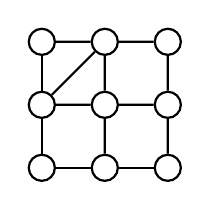
\begin{tikzpicture}[auto,
    specification/.style ={circle, draw, thick}, scale = 0.8]
   \node[specification] (A)  at (0,0)  {};
   \node[specification] (B)  at (1,0)  {};
   \node[specification] (C)  at (2,0)  {};
   \node[specification] (D)  at (0,1)  {};
   \node[specification] (E)  at (1,1)  {};
   \node[specification] (F)  at (2,1)  {};
   \node[specification] (G)  at (0,2)  {};
   \node[specification] (H)  at (1,2)  {};
   \node[specification] (I)  at (2,2)  {};

   \draw[thick] (A) to  (B);
   \draw[thick] (B) to  (C);
   \draw[thick] (D) to  (E);
   \draw[thick] (E) to  (F);
   \draw[thick] (G) to (H);
   \draw[thick] (H) to (I);
   \draw[thick] (A) to (D);
   \draw[thick] (B) to (E);
   \draw[thick] (C) to (F);
   \draw[thick] (D) to (G);
   \draw[thick] (E) to (H);
   \draw[thick] (F) to (I);
   \draw[thick] (D) to (H);

 \end{tikzpicture}
\end{minipage}\hfill
      C.
    \begin{minipage}{0.18\linewidth}
    \centering
    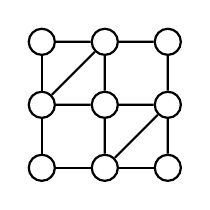
\begin{tikzpicture}[auto,
    specification/.style ={circle, draw, thick}, scale=0.8]
   \node[specification] (A)  at (0,0)  {};
   \node[specification] (B)  at (1,0)  {};
   \node[specification] (C)  at (2,0)  {};
   \node[specification] (D)  at (0,1)  {};
   \node[specification] (E)  at (1,1)  {};
   \node[specification] (F)  at (2,1)  {};
   \node[specification] (G)  at (0,2)  {};
   \node[specification] (H)  at (1,2)  {};
   \node[specification] (I)  at (2,2)  {};

   \draw[thick] (A) to  (B);
   \draw[thick] (B) to  (C);
   \draw[thick] (D) to  (E);
   \draw[thick] (E) to  (F);
   \draw[thick] (G) to (H);
   \draw[thick] (H) to (I);
   \draw[thick] (A) to (D);
   \draw[thick] (B) to (E);
   \draw[thick] (C) to (F);
   \draw[thick] (D) to (G);
   \draw[thick] (E) to (H);
   \draw[thick] (F) to (I);
   \draw[thick] (D) to (H);
   \draw[thick] (B) to (F);
 \end{tikzpicture}
\end{minipage}\hfill
      D.
    \begin{minipage}{0.18\linewidth}
    \centering
    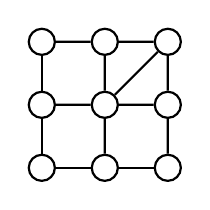
\begin{tikzpicture}[auto,
    specification/.style ={circle, draw, thick}, scale=0.8]
   \node[specification] (A)  at (0,0)  {};
   \node[specification] (B)  at (1,0)  {};
   \node[specification] (C)  at (2,0)  {};
   \node[specification] (D)  at (0,1)  {};
   \node[specification] (E)  at (1,1)  {};
   \node[specification] (F)  at (2,1)  {};
   \node[specification] (G)  at (0,2)  {};
   \node[specification] (H)  at (1,2)  {};
   \node[specification] (I)  at (2,2)  {};

   \draw[thick] (A) to  (B);
   \draw[thick] (B) to  (C);
   \draw[thick] (D) to  (E);
   \draw[thick] (E) to  (F);
   \draw[thick] (G) to (H);
   \draw[thick] (H) to (I);
   \draw[thick] (A) to (D);
   \draw[thick] (B) to (E);
   \draw[thick] (C) to (F);
   \draw[thick] (D) to (G);
   \draw[thick] (E) to (H);
   \draw[thick] (F) to (I);
   \draw[thick] (E) to (I);

 \end{tikzpicture}
\end{minipage}\hfill

\end{Ex}

\begin{Ex}
  以下4个图中,不可以一笔画成的是$\underline{\quad\quad}$。
  \vspace{0.5cm}

  A.
    \begin{minipage}{0.18\linewidth}
    \centering
    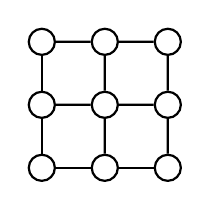
\begin{tikzpicture}[auto,
    specification/.style ={circle, draw, thick}, scale = 0.8]
   \node[specification] (A)  at (0,0)  {};
   \node[specification] (B)  at (1,0)  {};
   \node[specification] (C)  at (2,0)  {};
   \node[specification] (D)  at (0,1)  {};
   \node[specification] (E)  at (1,1)  {};
   \node[specification] (F)  at (2,1)  {};
   \node[specification] (G)  at (0,2)  {};
   \node[specification] (H)  at (1,2)  {};
   \node[specification] (I)  at (2,2)  {};

   \draw[thick] (A) to  (B);
   \draw[thick] (B) to  (C);
   \draw[thick] (D) to  (E);
   \draw[thick] (E) to  (F);
   \draw[thick] (G) to (H);
   \draw[thick] (H) to (I);
   \draw[thick] (A) to (D);
   \draw[thick] (B) to (E);
   \draw[thick] (C) to (F);
   \draw[thick] (D) to (G);
   \draw[thick] (E) to (H);
   \draw[thick] (F) to (I);
 \end{tikzpicture}
\end{minipage}\hfill
  B.
    \begin{minipage}{0.18\linewidth}
    \centering
    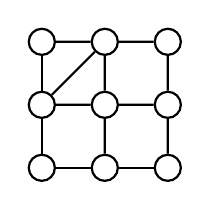
\begin{tikzpicture}[auto,
    specification/.style ={circle, draw, thick}, scale = 0.8]
   \node[specification] (A)  at (0,0)  {};
   \node[specification] (B)  at (1,0)  {};
   \node[specification] (C)  at (2,0)  {};
   \node[specification] (D)  at (0,1)  {};
   \node[specification] (E)  at (1,1)  {};
   \node[specification] (F)  at (2,1)  {};
   \node[specification] (G)  at (0,2)  {};
   \node[specification] (H)  at (1,2)  {};
   \node[specification] (I)  at (2,2)  {};

   \draw[thick] (A) to  (B);
   \draw[thick] (B) to  (C);
   \draw[thick] (D) to  (E);
   \draw[thick] (E) to  (F);
   \draw[thick] (G) to (H);
   \draw[thick] (H) to (I);
   \draw[thick] (A) to (D);
   \draw[thick] (B) to (E);
   \draw[thick] (C) to (F);
   \draw[thick] (D) to (G);
   \draw[thick] (E) to (H);
   \draw[thick] (F) to (I);
   \draw[thick] (D) to (H);

 \end{tikzpicture}
\end{minipage}\hfill
      C.
    \begin{minipage}{0.18\linewidth}
    \centering
    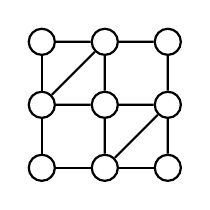
\begin{tikzpicture}[auto,
    specification/.style ={circle, draw, thick}, scale=0.8]
   \node[specification] (A)  at (0,0)  {};
   \node[specification] (B)  at (1,0)  {};
   \node[specification] (C)  at (2,0)  {};
   \node[specification] (D)  at (0,1)  {};
   \node[specification] (E)  at (1,1)  {};
   \node[specification] (F)  at (2,1)  {};
   \node[specification] (G)  at (0,2)  {};
   \node[specification] (H)  at (1,2)  {};
   \node[specification] (I)  at (2,2)  {};

   \draw[thick] (A) to  (B);
   \draw[thick] (B) to  (C);
   \draw[thick] (D) to  (E);
   \draw[thick] (E) to  (F);
   \draw[thick] (G) to (H);
   \draw[thick] (H) to (I);
   \draw[thick] (A) to (D);
   \draw[thick] (B) to (E);
   \draw[thick] (C) to (F);
   \draw[thick] (D) to (G);
   \draw[thick] (E) to (H);
   \draw[thick] (F) to (I);
   \draw[thick] (D) to (H);
   \draw[thick] (B) to (F);
 \end{tikzpicture}
\end{minipage}\hfill
      D.
    \begin{minipage}{0.18\linewidth}
    \centering
    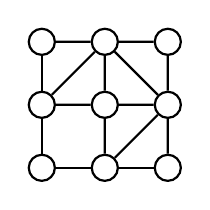
\begin{tikzpicture}[auto,
    specification/.style ={circle, draw, thick}, scale=0.8]
   \node[specification] (A)  at (0,0)  {};
   \node[specification] (B)  at (1,0)  {};
   \node[specification] (C)  at (2,0)  {};
   \node[specification] (D)  at (0,1)  {};
   \node[specification] (E)  at (1,1)  {};
   \node[specification] (F)  at (2,1)  {};
   \node[specification] (G)  at (0,2)  {};
   \node[specification] (H)  at (1,2)  {};
   \node[specification] (I)  at (2,2)  {};

   \draw[thick] (A) to  (B);
   \draw[thick] (B) to  (C);
   \draw[thick] (D) to  (E);
   \draw[thick] (E) to  (F);
   \draw[thick] (G) to (H);
   \draw[thick] (H) to (I);
   \draw[thick] (A) to (D);
   \draw[thick] (B) to (E);
   \draw[thick] (C) to (F);
   \draw[thick] (D) to (G);
   \draw[thick] (E) to (H);
   \draw[thick] (F) to (I);
   \draw[thick] (D) to (H);
   \draw[thick] (B) to (F);
   \draw[thick] (H) to (F);

 \end{tikzpicture}
\end{minipage}\hfill


\end{Ex}


\begin{Ex}
  以下4个图中,至少需要两笔才能画成的是$\underline{\quad\quad}$。
  \vspace{0.5cm}

  A.
    \begin{minipage}{0.18\linewidth}
    \centering
    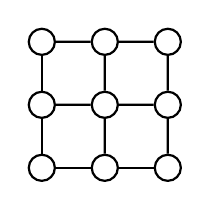
\begin{tikzpicture}[auto,
    specification/.style ={circle, draw, thick}, scale = 0.8]
   \node[specification] (A)  at (0,0)  {};
   \node[specification] (B)  at (1,0)  {};
   \node[specification] (C)  at (2,0)  {};
   \node[specification] (D)  at (0,1)  {};
   \node[specification] (E)  at (1,1)  {};
   \node[specification] (F)  at (2,1)  {};
   \node[specification] (G)  at (0,2)  {};
   \node[specification] (H)  at (1,2)  {};
   \node[specification] (I)  at (2,2)  {};

   \draw[thick] (A) to  (B);
   \draw[thick] (B) to  (C);
   \draw[thick] (D) to  (E);
   \draw[thick] (E) to  (F);
   \draw[thick] (G) to (H);
   \draw[thick] (H) to (I);
   \draw[thick] (A) to (D);
   \draw[thick] (B) to (E);
   \draw[thick] (C) to (F);
   \draw[thick] (D) to (G);
   \draw[thick] (E) to (H);
   \draw[thick] (F) to (I);
 \end{tikzpicture}
\end{minipage}\hfill
  B.
    \begin{minipage}{0.18\linewidth}
    \centering
    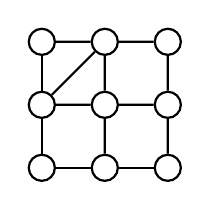
\begin{tikzpicture}[auto,
    specification/.style ={circle, draw, thick}, scale = 0.8]
   \node[specification] (A)  at (0,0)  {};
   \node[specification] (B)  at (1,0)  {};
   \node[specification] (C)  at (2,0)  {};
   \node[specification] (D)  at (0,1)  {};
   \node[specification] (E)  at (1,1)  {};
   \node[specification] (F)  at (2,1)  {};
   \node[specification] (G)  at (0,2)  {};
   \node[specification] (H)  at (1,2)  {};
   \node[specification] (I)  at (2,2)  {};

   \draw[thick] (A) to  (B);
   \draw[thick] (B) to  (C);
   \draw[thick] (D) to  (E);
   \draw[thick] (E) to  (F);
   \draw[thick] (G) to (H);
   \draw[thick] (H) to (I);
   \draw[thick] (A) to (D);
   \draw[thick] (B) to (E);
   \draw[thick] (C) to (F);
   \draw[thick] (D) to (G);
   \draw[thick] (E) to (H);
   \draw[thick] (F) to (I);
   \draw[thick] (D) to (H);

 \end{tikzpicture}
\end{minipage}\hfill
      C.
    \begin{minipage}{0.18\linewidth}
    \centering
    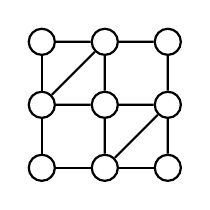
\begin{tikzpicture}[auto,
    specification/.style ={circle, draw, thick}, scale=0.8]
   \node[specification] (A)  at (0,0)  {};
   \node[specification] (B)  at (1,0)  {};
   \node[specification] (C)  at (2,0)  {};
   \node[specification] (D)  at (0,1)  {};
   \node[specification] (E)  at (1,1)  {};
   \node[specification] (F)  at (2,1)  {};
   \node[specification] (G)  at (0,2)  {};
   \node[specification] (H)  at (1,2)  {};
   \node[specification] (I)  at (2,2)  {};

   \draw[thick] (A) to  (B);
   \draw[thick] (B) to  (C);
   \draw[thick] (D) to  (E);
   \draw[thick] (E) to  (F);
   \draw[thick] (G) to (H);
   \draw[thick] (H) to (I);
   \draw[thick] (A) to (D);
   \draw[thick] (B) to (E);
   \draw[thick] (C) to (F);
   \draw[thick] (D) to (G);
   \draw[thick] (E) to (H);
   \draw[thick] (F) to (I);
   \draw[thick] (D) to (H);
   \draw[thick] (B) to (F);
 \end{tikzpicture}
\end{minipage}\hfill
      D.
    \begin{minipage}{0.18\linewidth}
    \centering
    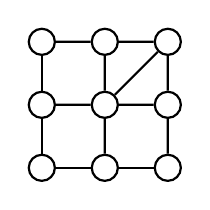
\begin{tikzpicture}[auto,
    specification/.style ={circle, draw, thick}, scale=0.8]
   \node[specification] (A)  at (0,0)  {};
   \node[specification] (B)  at (1,0)  {};
   \node[specification] (C)  at (2,0)  {};
   \node[specification] (D)  at (0,1)  {};
   \node[specification] (E)  at (1,1)  {};
   \node[specification] (F)  at (2,1)  {};
   \node[specification] (G)  at (0,2)  {};
   \node[specification] (H)  at (1,2)  {};
   \node[specification] (I)  at (2,2)  {};

   \draw[thick] (A) to  (B);
   \draw[thick] (B) to  (C);
   \draw[thick] (D) to  (E);
   \draw[thick] (E) to  (F);
   \draw[thick] (G) to (H);
   \draw[thick] (H) to (I);
   \draw[thick] (A) to (D);
   \draw[thick] (B) to (E);
   \draw[thick] (C) to (F);
   \draw[thick] (D) to (G);
   \draw[thick] (E) to (H);
   \draw[thick] (F) to (I);
   \draw[thick] (E) to (I);

 \end{tikzpicture}
\end{minipage}\hfill

\end{Ex}


\begin{Ex}
  以下4个图中,至少需要三笔才能画成的是$\underline{\quad\quad}$。
  \vspace{0.5cm}

  A.
    \begin{minipage}{0.18\linewidth}
    \centering
    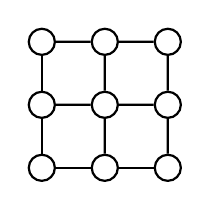
\begin{tikzpicture}[auto,
    specification/.style ={circle, draw, thick}, scale = 0.8]
   \node[specification] (A)  at (0,0)  {};
   \node[specification] (B)  at (1,0)  {};
   \node[specification] (C)  at (2,0)  {};
   \node[specification] (D)  at (0,1)  {};
   \node[specification] (E)  at (1,1)  {};
   \node[specification] (F)  at (2,1)  {};
   \node[specification] (G)  at (0,2)  {};
   \node[specification] (H)  at (1,2)  {};
   \node[specification] (I)  at (2,2)  {};

   \draw[thick] (A) to  (B);
   \draw[thick] (B) to  (C);
   \draw[thick] (D) to  (E);
   \draw[thick] (E) to  (F);
   \draw[thick] (G) to (H);
   \draw[thick] (H) to (I);
   \draw[thick] (A) to (D);
   \draw[thick] (B) to (E);
   \draw[thick] (C) to (F);
   \draw[thick] (D) to (G);
   \draw[thick] (E) to (H);
   \draw[thick] (F) to (I);
 \end{tikzpicture}
\end{minipage}\hfill
  B.
    \begin{minipage}{0.18\linewidth}
    \centering
    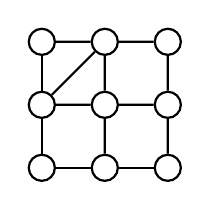
\begin{tikzpicture}[auto,
    specification/.style ={circle, draw, thick}, scale = 0.8]
   \node[specification] (A)  at (0,0)  {};
   \node[specification] (B)  at (1,0)  {};
   \node[specification] (C)  at (2,0)  {};
   \node[specification] (D)  at (0,1)  {};
   \node[specification] (E)  at (1,1)  {};
   \node[specification] (F)  at (2,1)  {};
   \node[specification] (G)  at (0,2)  {};
   \node[specification] (H)  at (1,2)  {};
   \node[specification] (I)  at (2,2)  {};

   \draw[thick] (A) to  (B);
   \draw[thick] (B) to  (C);
   \draw[thick] (D) to  (E);
   \draw[thick] (E) to  (F);
   \draw[thick] (G) to (H);
   \draw[thick] (H) to (I);
   \draw[thick] (A) to (D);
   \draw[thick] (B) to (E);
   \draw[thick] (C) to (F);
   \draw[thick] (D) to (G);
   \draw[thick] (E) to (H);
   \draw[thick] (F) to (I);
   \draw[thick] (D) to (H);

 \end{tikzpicture}
\end{minipage}\hfill
      C.
    \begin{minipage}{0.18\linewidth}
    \centering
    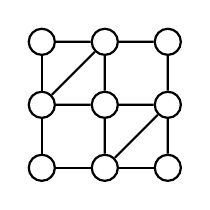
\begin{tikzpicture}[auto,
    specification/.style ={circle, draw, thick}, scale=0.8]
   \node[specification] (A)  at (0,0)  {};
   \node[specification] (B)  at (1,0)  {};
   \node[specification] (C)  at (2,0)  {};
   \node[specification] (D)  at (0,1)  {};
   \node[specification] (E)  at (1,1)  {};
   \node[specification] (F)  at (2,1)  {};
   \node[specification] (G)  at (0,2)  {};
   \node[specification] (H)  at (1,2)  {};
   \node[specification] (I)  at (2,2)  {};

   \draw[thick] (A) to  (B);
   \draw[thick] (B) to  (C);
   \draw[thick] (D) to  (E);
   \draw[thick] (E) to  (F);
   \draw[thick] (G) to (H);
   \draw[thick] (H) to (I);
   \draw[thick] (A) to (D);
   \draw[thick] (B) to (E);
   \draw[thick] (C) to (F);
   \draw[thick] (D) to (G);
   \draw[thick] (E) to (H);
   \draw[thick] (F) to (I);
   \draw[thick] (D) to (H);
   \draw[thick] (B) to (F);
 \end{tikzpicture}
\end{minipage}\hfill
      D.
    \begin{minipage}{0.18\linewidth}
    \centering
    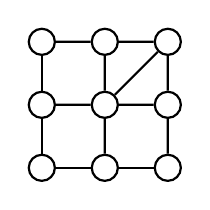
\begin{tikzpicture}[auto,
    specification/.style ={circle, draw, thick}, scale=0.8]
   \node[specification] (A)  at (0,0)  {};
   \node[specification] (B)  at (1,0)  {};
   \node[specification] (C)  at (2,0)  {};
   \node[specification] (D)  at (0,1)  {};
   \node[specification] (E)  at (1,1)  {};
   \node[specification] (F)  at (2,1)  {};
   \node[specification] (G)  at (0,2)  {};
   \node[specification] (H)  at (1,2)  {};
   \node[specification] (I)  at (2,2)  {};

   \draw[thick] (A) to  (B);
   \draw[thick] (B) to  (C);
   \draw[thick] (D) to  (E);
   \draw[thick] (E) to  (F);
   \draw[thick] (G) to (H);
   \draw[thick] (H) to (I);
   \draw[thick] (A) to (D);
   \draw[thick] (B) to (E);
   \draw[thick] (C) to (F);
   \draw[thick] (D) to (G);
   \draw[thick] (E) to (H);
   \draw[thick] (F) to (I);
   \draw[thick] (E) to (I);

 \end{tikzpicture}
\end{minipage}\hfill

\end{Ex}

%%% Local Variables:
%%% mode: latex
%%% TeX-master: "book"
%%% End:
